\begin{frame}
\frametitle{Two-dimensional case - Setup}
Consider $D=[-1,1]^2$ and the SDE
\begin{equation*}
\left \{
\begin{aligned}
	dX(t) &= f(X(t)) dt + g(X(t))dW(t), && 0 < t \leq T, \\
	X(0)  &= X_0, && X_0 \in D.
\end{aligned} \right .
\end{equation*}
Setting:
\begin{itemize}
	\item Mixed boundary conditions, \\
	\item $f = 0$ $\to$ pure Brownian motion.
\end{itemize}
\underline{Goal}. Verify the weak order of convergence of DEM and CEM. \\
\underline{Reference solution}. Solution of PDE's with FEM.
\end{frame}

\begin{frame}
\frametitle{Two-dimensional case - Results}
\begin{figure}[t]
    \centering
    \begin{subfigure}{0.49\linewidth}
        \centering
        \resizebox{1\linewidth}{!}{% This file was created by matlab2tikz.
%
%The latest updates can be retrieved from
%  http://www.mathworks.com/matlabcentral/fileexchange/22022-matlab2tikz-matlab2tikz
%where you can also make suggestions and rate matlab2tikz.
%
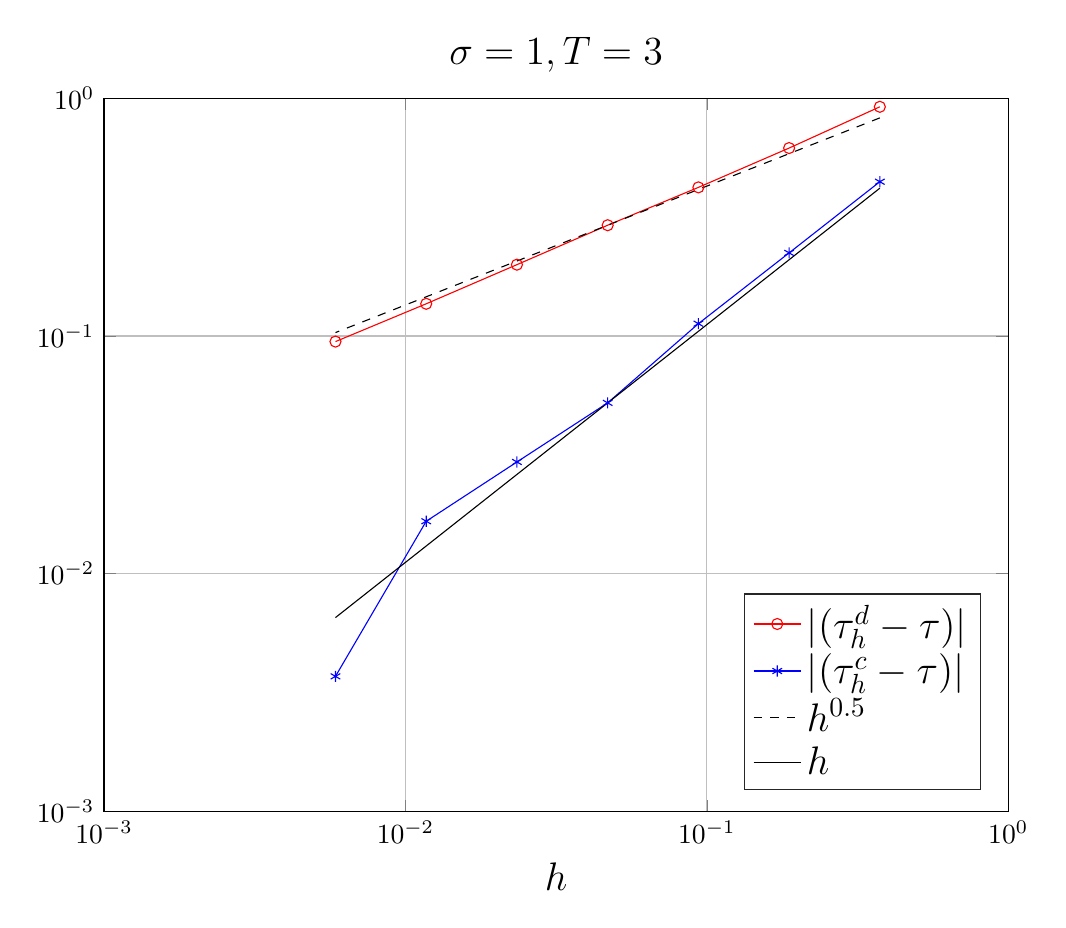
\begin{tikzpicture}

\begin{axis}[%
width=4.521in,
height=3.566in,
at={(0.758in,0.481in)},
scale only axis,
title={$\sigma = 1, T = 3$},
title style = {font=\Large},
xmode=log,
xmin=0.001,
xmax=1,
xminorticks=false,
xlabel={$h$},
xlabel style={font=\Large},
xmajorgrids,
ymode=log,
ymin=0.001,
ymax=1,
yminorticks=false,
ymajorgrids,
axis background/.style={fill=white},
legend pos = south east,
legend style={legend cell align=left,align=left,draw=white!15!black,font=\Large}
]
\addplot [color=red,solid,mark=o,mark options={solid}]
  table[row sep=crcr]{%
0.375	0.920558951920583\\
0.1875	0.617333951920583\\
0.09375	0.421846451920583\\
0.046875	0.292363639420583\\
0.0234375	0.199588639420583\\
0.01171875	0.136614420670583\\
0.005859375	0.0947198894205827\\
};
\addlegendentry{$|\E(\tau_h^d - \tau)|$};

\addplot [color=blue,solid,mark=asterisk,mark options={solid}]
  table[row sep=crcr]{%
0.375	0.445546451920583\\
0.1875	0.223658951920583\\
0.09375	0.112677701920583\\
0.046875	0.0523214519205826\\
0.0234375	0.0295214519205826\\
0.01171875	0.0166261394205827\\
0.005859375	0.00370153004558271\\
};
\addlegendentry{$|\E(\tau_h^c - \tau)|$};

\addplot [color=black,dashed]
  table[row sep=crcr]{%
0.375	0.82692924802669\\
0.1875	0.584727278841165\\
0.09375	0.413464624013345\\
0.046875	0.292363639420583\\
0.0234375	0.206732312006673\\
0.01171875	0.146181819710291\\
0.005859375	0.103366156003336\\
};
\addlegendentry{$h^{0.5}$};

\addplot [color=black,solid]
  table[row sep=crcr]{%
0.375	0.418571615364661\\
0.1875	0.20928580768233\\
0.09375	0.104642903841165\\
0.046875	0.0523214519205826\\
0.0234375	0.0261607259602913\\
0.01171875	0.0130803629801456\\
0.005859375	0.00654018149007282\\
};
\addlegendentry{$h$};

\end{axis}
\end{tikzpicture}%
 }  
        \caption{Approximation of $\tau$}
        \label{fig:KillOneDPhi}
    \end{subfigure}
    \begin{subfigure}{0.49\linewidth}
        \centering
        \resizebox{1\linewidth}{!}{% This file was created by matlab2tikz.
%
%The latest updates can be retrieved from
%  http://www.mathworks.com/matlabcentral/fileexchange/22022-matlab2tikz-matlab2tikz
%where you can also make suggestions and rate matlab2tikz.
%
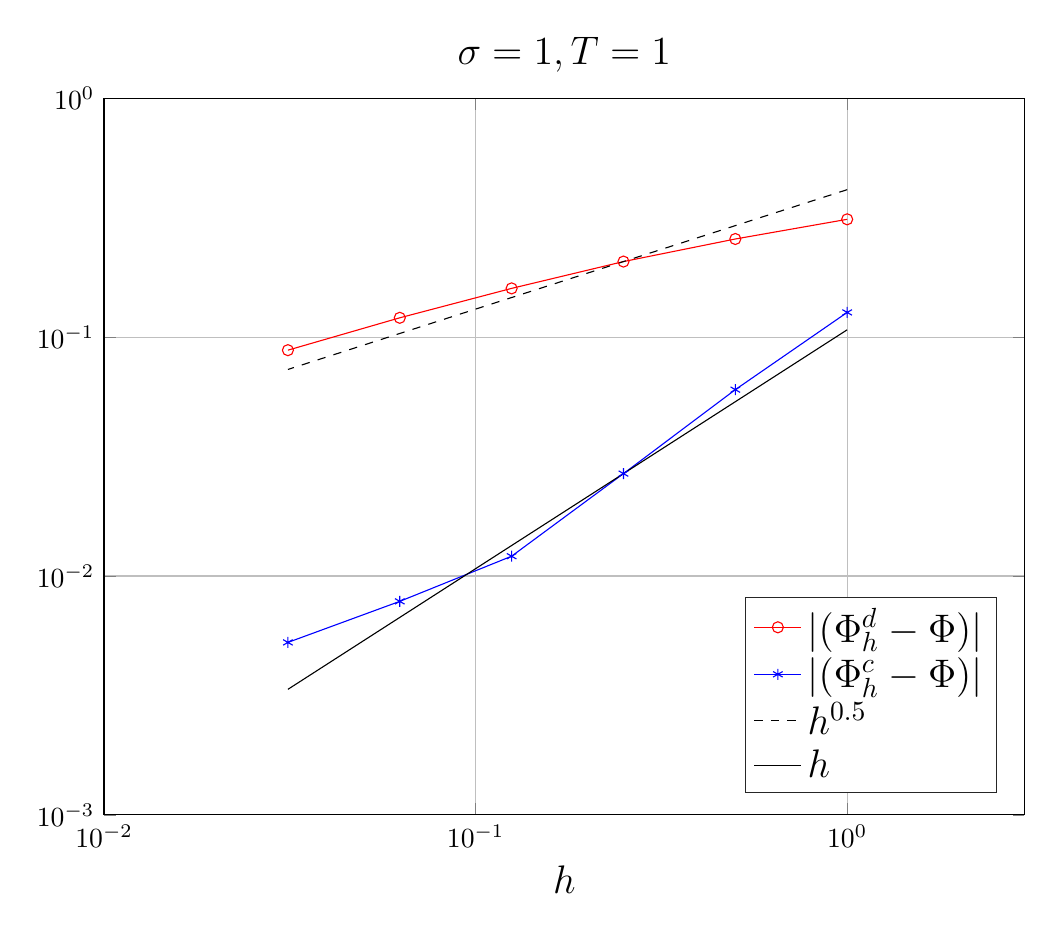
\begin{tikzpicture}

\begin{axis}[%
width=4.602in,
height=3.583in,
at={(0.772in,0.484in)},
scale only axis,
title={$\sigma = 1, T = 1$},
title style = {font=\Large},
xmode=log,
xmin=0.01,
xmax=3,
xminorticks=false,
xlabel={$h$},
xlabel style={font=\Large},
xmajorgrids,
ymode=log,
ymin=0.001,
ymax=1,
yminorticks=false,
ymajorgrids,
axis background/.style={fill=white},
legend pos = south east,
legend style={legend cell align=left,align=left,draw=white!15!black,font=\Large}
]
\addplot [color=red,solid,mark=o,mark options={solid}]
  table[row sep=crcr]{%
1	0.31134162505938\\
0.5	0.25753162505938\\
0.25	0.20716162505938\\
0.125	0.15999162505938\\
0.0625	0.12047162505938\\
0.03125	0.0881916250593803\\
};
\addlegendentry{$|\E(\Phi_h^d - \Phi)|$};

\addplot [color=blue,solid,mark=asterisk,mark options={solid}]
  table[row sep=crcr]{%
1	0.12689162505938\\
0.5	0.0602816250593803\\
0.25	0.0268316250593803\\
0.125	0.0121016250593803\\
0.0625	0.00783162505938029\\
0.03125	0.00527162505938028\\
};
\addlegendentry{$|\E(\Phi_h^c - \Phi)|$};

\addplot [color=black,dashed]
  table[row sep=crcr]{%
1	0.41432325011876\\
0.5	0.292970779762226\\
0.25	0.20716162505938\\
0.125	0.146485389881113\\
0.0625	0.10358081252969\\
0.03125	0.0732426949405564\\
};
\addlegendentry{$h^{0.5}$};

\addplot [color=black,solid]
  table[row sep=crcr]{%
1	0.107326500237521\\
0.5	0.0536632501187606\\
0.25	0.0268316250593803\\
0.125	0.0134158125296902\\
0.0625	0.00670790626484508\\
0.03125	0.00335395313242254\\
};
\addlegendentry{$h$};

\end{axis}
\end{tikzpicture}%
 }  
        \caption{Approximation of $\Phi$}
        \label{fig:ReflectOneDPhi}
    \end{subfigure}    
    \caption{Results for the two-dimensional case.}
\end{figure}
\end{frame}
